\documentclass[12pt]{article}\usepackage[english]{babel}\usepackage{xcolor}\usepackage[hmargin=1in,vmargin=1in]{geometry}\usepackage{amsmath}\usepackage{unicode-math}\usepackage[round,sort,comma]{natbib}\bibliographystyle{apa}\usepackage{setspace}\let\oldbibitem\bibitem\renewcommand{\bibitem}[2][]{\oldbibitem[#1]{#2} \setlength{\itemsep}{0pt}}\usepackage{graphicx}\usepackage{caption}\usepackage{subcaption}\usepackage[colorlinks=true, allcolors=blue]{hyperref}\usepackage{float}\usepackage{booktabs}\usepackage{advdate}\AdvanceDate[-1]\usepackage{titlesec}\newcommand{\addperiod}[1]{#1.$\;$}\titlespacing{\section}{0pt}{0.5\parskip}{-\parskip}\titleformat{\subsection}[runin]{\normalsize\bfseries}{\thesubsection}{1em}{\addperiod}\titleformat{\subsubsection}[runin]{\normalfont\normalsize\itshape}{\thesubsubsection}{1em}{\addperiod}\titlespacing{\subsubsection}{14pt plus 4pt minus 2pt}{0.5\parskip}{-\parskip}\setlength{\parindent}{1em}\makeatletter\g@addto@macro \normalsize {\setlength\abovedisplayskip{3pt plus 5pt minus 2pt}\setlength\belowdisplayskip{3pt plus 5pt minus 2pt}}\makeatother\newcommand{\comment}[1]{}\usepackage{tikz}\usetikzlibrary{positioning, shapes}  \begin{document}\pagenumbering{gobble}\begin{center}{\fontsize{16}{16}\selectfont\bfseries \texttt{reproduce.work}: A framework to facilitate cross-platform computational reproducibility in scientific publishing}\\\vspace{5mm}\begin{table}[!ht]\begin{center}\begin{tabular}{c c }\shortstack{ Alex P. Miller \\USC Marshall School of Business \\alex.miller@marshall.usc.edu }\end{tabular}\end{center}\end{table}\vspace{5mm}\emph{Last updated: \today}\vspace{4mm}\hyphenpenalty=10000 \exhyphenpenalty=10000\abstract{In metascience, computational reproduction is the process of reproducing the results of a scientific paper
using the data and code provided by the authors of the paper. This subject sits within the broader context of 
``reproducibility" in scientific  research, which has been core to the philosophy of science for decades. However, 
the practice of science has fallen woefully short of meeting even basic standards toward true and widespread 
reproducibility. In this project, we focus primarily on addressing the narrow problem of computational reproducibility. 
We propose a framework for facilitating computational reproducibility in scientific publishing, which we call 
reproduce.work. The reproducibility standards are designed to be cross-platform and to work with any programming language, 
though our first working software interfaces are in Python.
We highlight the distinction between open and reproducibile practices and show how our software framework encourages 
both simultaneously. The results of this very paper can be reproduced on any machine that can execute a containerized 
image using the reproduce.work workflow. We conclude by discussing the potential of the framework for improving rigor 
and fidelity of computational science for both producers and consumers of published work.
}\\\vspace{2cm}{\scriptsize \noindent Notes: reproduce.work/v0.0.1  \raisebox{-1mm}{
\includegraphics[width=5mm]{../../../../img/logo.png}} }\hyphenpenalty=50 \exhyphenpenalty=50\vspace{10mm}\end{center}\newpage\pagenumbering{arabic}\setcounter{page}{1} \doublespacing 

\hypertarget{introduction}{%
\section{Introduction}\label{introduction}}

An increasing number of scientists across various disciplines are calling for heightened standards of reproducibility in published work   \citep{lindsay2023plea,mcnutt2014}. From biomedical research and computer science to management, psychology, and economics, the scientific community is grappling with the challenges of ensuring that published scientific work is verifiable and trustworthy \citep{cancer2021Reproducibility,christensen2018transparency,hutson2018artificial,davis2023replication}.  Several scholars have described the current state of affairs as an epistemological ``crisis'' in the core of science  \citep{dreber2019statistical,dougherty2008epistemological,earp2015replication,gelman2016statistical}. 
In its most dramatic form, high profile accusations of data fabrication have led to \verb,$,25 million dollar lawsuits and the resignation of a university presidents \citep{nytimesHarvardProfessor, stanforddailyReviewFound}. 

A more mundane but pervasive manifestation of epistemological precarity is the fact that most scientific papers are not reproducible to even the lowest degree \citep{gomes2022don,tenopir2020data}. A low percentage of published papers claim to share their data and code; of those that do, many fail to follow through or even respond to inquiries \citep{tenopir2011data}. Even when good faith efforts are made to share data and code, the vagaries of software development and the complexity of scientific code make it difficult to reproduce results across time, space, and computing environments.
Unfortunately for the incentives of honest scientists, \cite{serragarciagneezy2021} find that nonreplicable publications are cited about twice as much as replicable ones. The problem is exacerbated by the fact that many scientists do not understand the nature of statistical inference and human's innate tendency to search for patterns in data \citep{gelman2016statistical,ioannidis2009repeatability}.
The low bar for publication in many scientific journals, has resulted in a literature that is rife with false positives and irreproducible results \citep{ioannidis2005most,ioannidis2017power}.

In metascience, computational reproduction is the process of reproducing the results of a scientific paper using the data and code provided by the authors of the paper. This subject sits within the broader context of ``reproducibility'' in scientific  research, which is the idea that scientific results should be reproducible by other scientists (or anyone interested, for that matter). Concepts around reproducibility have been core to the philosophy of science for decades, but several aspects of the scientific method have been challenged by recent developments. On top of the outright fraud and misconduct that is apparently common, there are more subtle forms research malpractice and human error that are known to pervade the published scientific literature as well, in the form of selective publication and $p$-hacking described above. On top of all this, the complexity of scientific code and restrictiveness of many data sharing agreements means that most published scientific results are not reproducible to even the lowest degree. 
Among those concerned about reproducibility on all fronts, this has led to a call for heightened standards of reproducibility in scientific research. 

To this end, we introduce a simple framework for achieving and demonstrating computational reproducibility, referred to as \texttt{reproduce.work}. The associated scientific development kit is designed to facilitate production of reproducible scientific computing projects by default. It features a full-featured computing environment (enabled by containerization) that is compatible with essentially any existing scientific workflow. The framework also features a suite of software that facilitates the publication of standardized computational reports with structured metadata. The framework is designed to be as simple as possible while accommodating a wide variety of scientific output. As a proof-of-concept version 0.0.1 example of this framework, the source code for this paper and the full stack containerized environment used to produce it are open source and can be found \href{https://github.com/reproduce-work/reproduce-work}{here}\footnote{\href{https://github.com/reproduce-work/reproduce-work}{https://github.com/reproduce-work/reproduce-work}} run and in any modern computing environment. 

\hypertarget{background}{%
\section{Background}\label{background}}

reproducibility, in the context of the philosophy of science, metascience, and empiricism, refers to the ability of a scientific study or experiment to be independently repeated under the same conditions to verify the original results. It is a cornerstone of the scientific method, ensuring that findings are not anomalous or products of error or bias. The goal of reproduction is ensure that science is built on consistent and generalizable truths. The emphasis on reproducibility underscores the importance of transparency, rigor, and skepticism in the pursuit of knowledge, as recent developments in the broader scientific community have prompted widespread introspection within about practices, methodologies, and the reliability of published findings.

While a unified concept at its core, the concept of reproducibility can manifest in various forms based on the specific domain or the nature of the scientific investigation. Here we theorize about the different dimensions of reproducibility:

\begin{itemize}
\itemsep -0.2em
\item Direct replicability (i.e., reproducibility):  The most straightforward form of replication; the aim is to determine if the same results emerge under virtually identical conditions. Depending on the research methodology, this may take one of several forms:

\begin{itemize}
\itemsep -0.2em
\item Computational reproducibility: This involves rerunning analyses with the original code and dataset.
\item Procedural reproducibility: where researchers attempt to recreate the original study as closely as possible using the same procedures, materials, and subjects or subject pool (if applicable).
\end{itemize}
\item Conceptual replicability (i.e., generalizability, mere ``replicability''): Rather than mirroring the original study exactly, conceptual reproduction involves testing the same underlying hypothesis but with different methods or procedures. This type of reproduction examines the robustness of the original findings and whether they can be generalized across different contexts or approaches.
\end{itemize}

While conceptual reproduction is obviously core to the scientific method, the focus of this project will be limited to computational reproducibility. We believe that computational reproducibility is a small but necessary first step toward a world where scientific results are verifiable. Given the low bars of existing standards in scientific practice, we beleive this project and the ideas put forward here have potential as the seed of a growing culture of scientific rigor and transparency.

\hypertarget{barriers-to-computational-reproduction}{%
\subsection{Barriers to computational reproduction}\label{barriers-to-computational-reproduction}}

We highlight several challenges to computational reproduction that are not necessarily unique to but are common in scientific research. 
\textbf{Lack of documentation},
\textbf{Platform dependence},
\textbf{Code complexity},
\textbf{Lack of independent verification}, and
\textbf{Data availability}.

The last of these challenges will always remain relevant to some degree. However, this project is based on notion that the first four challenges are all amenable to software solutions to some degree. The purpose of this project is to develop a framework for computational reproducibility that is designed to overcome the challenges of poor documentation, platform dependence, and code complexity, and lack of verification. 

\hypertarget{related-initiatives}{%
\subsection{Related initiatives}\label{related-initiatives}}

\hypertarget{existing-environments-for-scientific-publishing}{%
\subsubsection{Existing environments for scientific publishing}\label{existing-environments-for-scientific-publishing}}

There exist a number of projects with similar aims to this one. We highlight the \href{https://jupyter.org/}{Jupyter} ecosystem --- including 
the \href{https://jupyterbook.org/en/stable/content/myst.html}{MyST Markdown} and \href{https://nbdev.fast.ai/}{nbdev} projects that both facilitate well-documented scientific software \citep{rule2019ten}. The \href{https://rstudio.com/}{RStudio} and 
 \href{https://rmarkdown.rstudio.com/}{RMarkdown} computing environments are also widely used tools in statistical computing that have features that encourage the alignment of scientific computing and publishing. (Also see \href{https://mine-cetinkaya-rundel.github.io/improve-repro-workflow-reproducibilitea-2020/}{this example} of an R-based workflow.) These projects are designed to facilitate the production of scientific reports that are both human-readable and computationally reproducible. However, these projects have some restrictions with respect to the software they are able to execute and, further, they have no mechanism or standards for verifying that the results reported in the published document are indeed reproducible. This is not a criticism, by any means; the reproduce.work project builds on these concepts but with objectives that are optimized for a specific vision of computational reproducibility. 

The reality, however, is that very few scientists have a reproducible ``environment'' in any meaningful sense of that word from the perspective of scientific computing. Most scientists use a variety of software packages and programming languages to conduct their research. They may copy and paste data between applications, such as R or Stata or MATLAB, and they may use a variety of software platforms to compose their reports. Overleaf is a popular SaaS {\LaTeX}   engine; Google Docs and Microsoft Word are a popular word processors. As such, the default environment is the ad hoc environment, which is to say that the default environment for most published scientists is no environment at all.

\hypertarget{existing-efforts-around-reproducible-science}{%
\subsubsection{Existing efforts around reproducible science}\label{existing-efforts-around-reproducible-science}}

We wish to highlight the efforts of the \href{http://rescience.github.io/}{The ReScience Initiative}, which is an effort to publish the results of independent replications. They have developed a set of standards for publishing replications of scientific results, with a particular focus on reproducing projects in computational neuroscience, robotics, computer science, and bioinformatics \citep{ReScience}. We believe there is significant room for improvement of reproduction across many domains of scientific research, particularly in the economic and social sciences, including those of core business research such as management, marketing, and information systems. We hope our project can find its own niche of scientific adopters and view our efforts merely as a complement to the excellent work going on in other areas of science.\footnote{Note that our disinction between ``direct'' and ``conceptual replication'' map on to the convention ReScience uses to distinguish between ``reproduction'' and ``replication'' \citep{ReScience}.}




In this project, we highlight our principle aim for the release versions revolve around \textit{reproduction} in this sense of the word, as should be implied by our definition of \textit{direct replication} above. However, we do also believe our framework may be used to also facilitate replication and meta-analysis in the future as well. We leave this as an open question for future versions of this project.

\hypertarget{difference-between-open-science-and-reproducible-science}{%
\subsubsection{Difference between open science and reproducible science}\label{difference-between-open-science-and-reproducible-science}}

We believe there is a case to made for distinguishing between the goals of ``opennness'' and ``reproducibility''. 
There do exist efforts around ``open science'', which are related but distinct from reproducible science. See OSF's \href{https://osf.io/tvyxz/}{``Badges to Acknowledge Open Practices
``}, for example, which is an intitiative aimed to give badges to projects that meet certain standards of openness. The Open Science Framework as a whole is, of course, a great example of an large and distributed effort to encourage open science. Note however the important distinction between reproducible and open science objectives.

As mentioned above, a reproducible project is one for which at least one independent party has verified that the stated results match the actual results of the code and data provided by the authors. It is in principle quite easy to publish an ``open'' science project without clearing this bar. For example, one could publish a project with open data and code, but the code could be incorrect or the data could be manipulated. (It is also possible, in principle, for there to be reproducible projects that are not open, or selectively open depending on the access preferences of the publishing authors.)
This is not to say that open science is not a worthy goal; it is. However, we believe that reproducible science is a different objective and one that is also worth aiming for.

\hypertarget{bad-actors}{%
\subsubsection{Bad actors}\label{bad-actors}}

Our project is no panacea for the problem of human error and fraud. As such, it worth asking whether the benefits of reproducible science are worth the effort. The primary aim of this project is to help make reproducibility a default standard in relevent sectors of scientific publishing by developing user-centric software that lowers the bar to reproducibily scientific development. However, it is worth noting that even in the worst-case scenarios, where a researcher is attempting to commit fraud or deception, we believe a standardized reproducibility framework, combined with open science, can offer some benefits for the aims of science as a whole. These include:

\begin{itemize}
\itemsep -0.2em
\item Traceability: Even if someone tries to abuse the system, the transparent nature of the framework ensures that their actions can be traced back and audited.
\item Standardized Inspection: Since everyone adheres to the same standard, it becomes easier to inspect, review, and identify anomalies.
\item Flexibility: The modular nature of the design means it can be adapted or updated to counter new threats or abuses as they emerge.
\end{itemize}




\hypertarget{software-}{%
\section{Software: \texttt{reproduce.work}}\label{software-}}

The preceding conversation highlights the need for a new paradigm for scientific computing in publishing. One that prioritizes both producers and consumers of scientific documents, with an aim specifically toward facilitating computational reproducibility. This allows us to introduce the alpha v0.0.1 version of the \texttt{reproduce.work} framework, which we do so briefly here.

\hypertarget{section}{%
\subsection{\texttt{reproduce.work}}\label{section}}

At the heart of the \texttt{reproduce.work} ecosystem is a commitment to value of structured metadata. The primary contribution of the reproduce.work standards framework is its ability to augment published scientific work with a static ledger of structured metadata that facilitates human traceability of results and computational reproducibility. This is a simple idea, but it has profound implications for the way that scientific reports are produced and published.

The concept is visualized in Figure \ref{fig:comp}. In this diagram, we communicate several key aspects of the way the \texttt{reproduce.work} is envisioned to work. One key factor the software tools, starting with the \texttt{sci-dev-kit}, which facilitate  reproducible, self-documenting scientific reports. The mechanism for verifying reproducibility consists of a set of standards that can be checked and cross referenced depending on aspects of the metadata embedded in the report.

The nature of the metadata is also represented in Figure \ref{fig:tracked}, which we compare to existing paradigms for scientific development. In the current paradigm, scientific computing and publishing are separate processes that some software allow to be integrated for users; however this seemlessness makes it difficult to exactly which data is important for publication and which is incidental.  In the \texttt{tracked} model, the data and code are tracked in a way that allows for easy verification and traceability of reported scientific results with structured metadata.


\begin{figure}[h]
\centering
\caption{\texttt{reproduce.work} is a set of software and standards for scientific publishing}
\label{fig:comp}
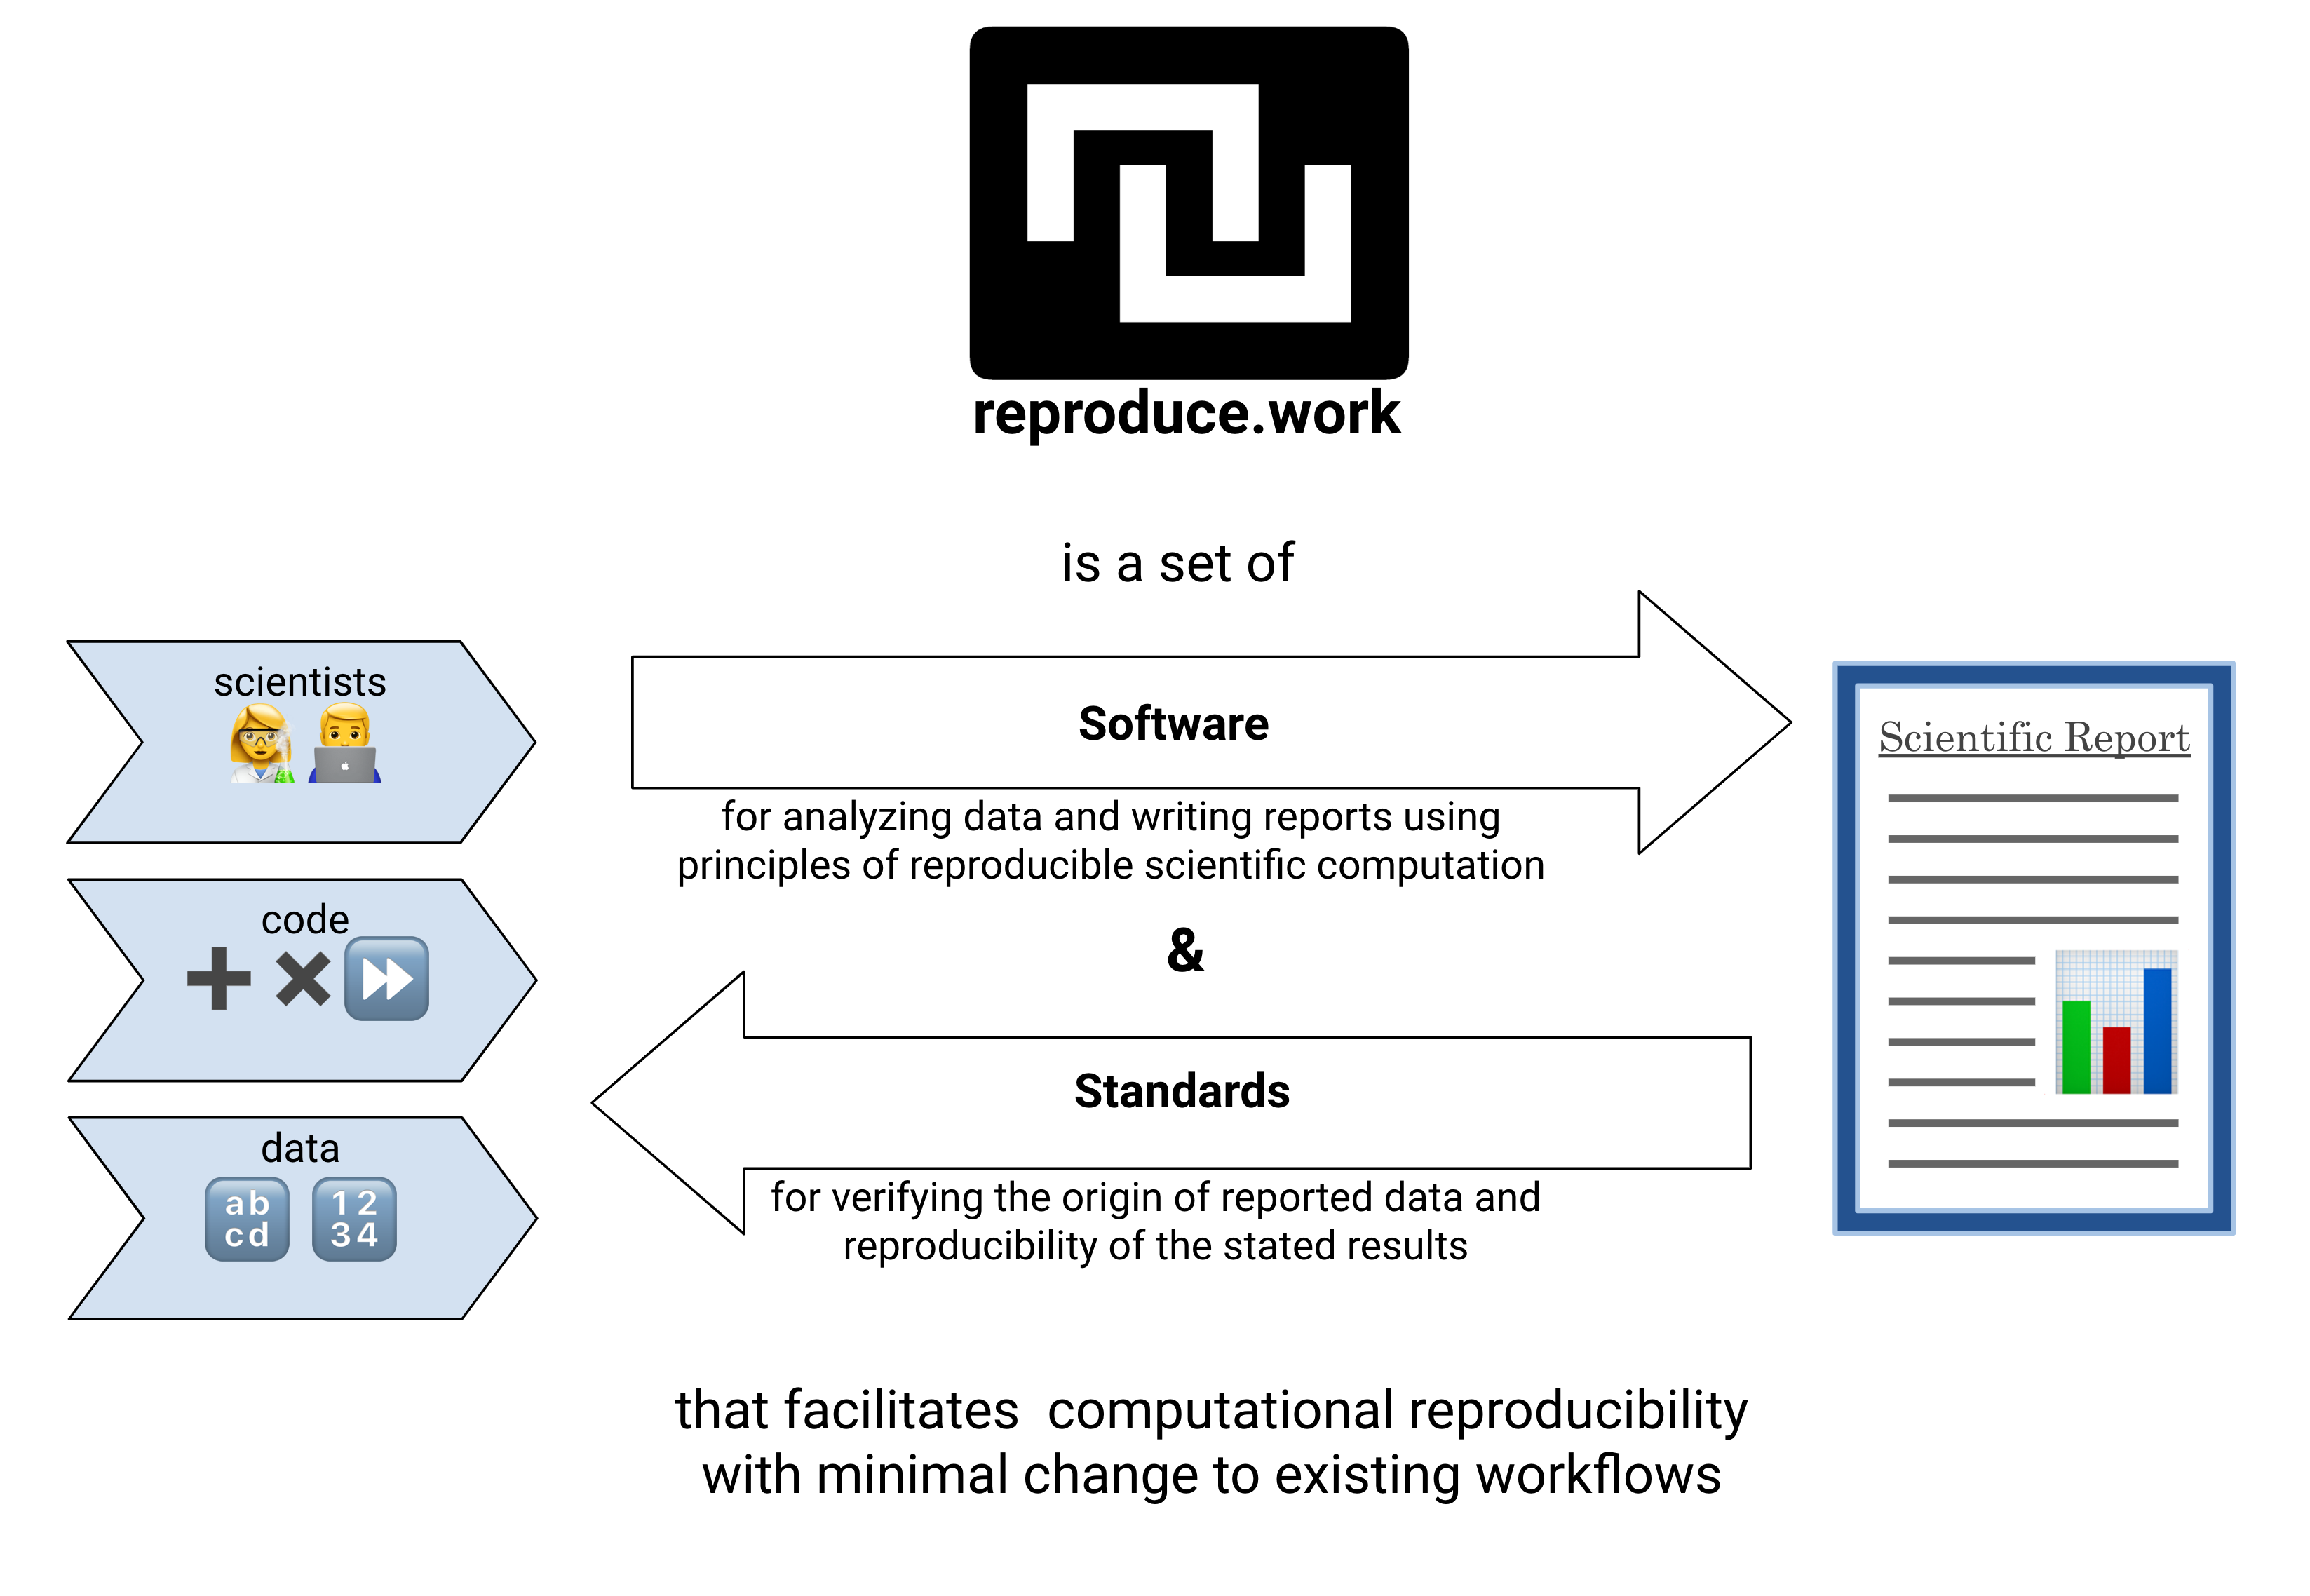
\includegraphics[width=.85\textwidth]{../../../../img/reproduce_is.png}
\end{figure}

\begin{figure}[h]
\centering
\caption{Comparison of linear vs. tracked models of scientific development}
\label{fig:tracked}
\hspace{2mm}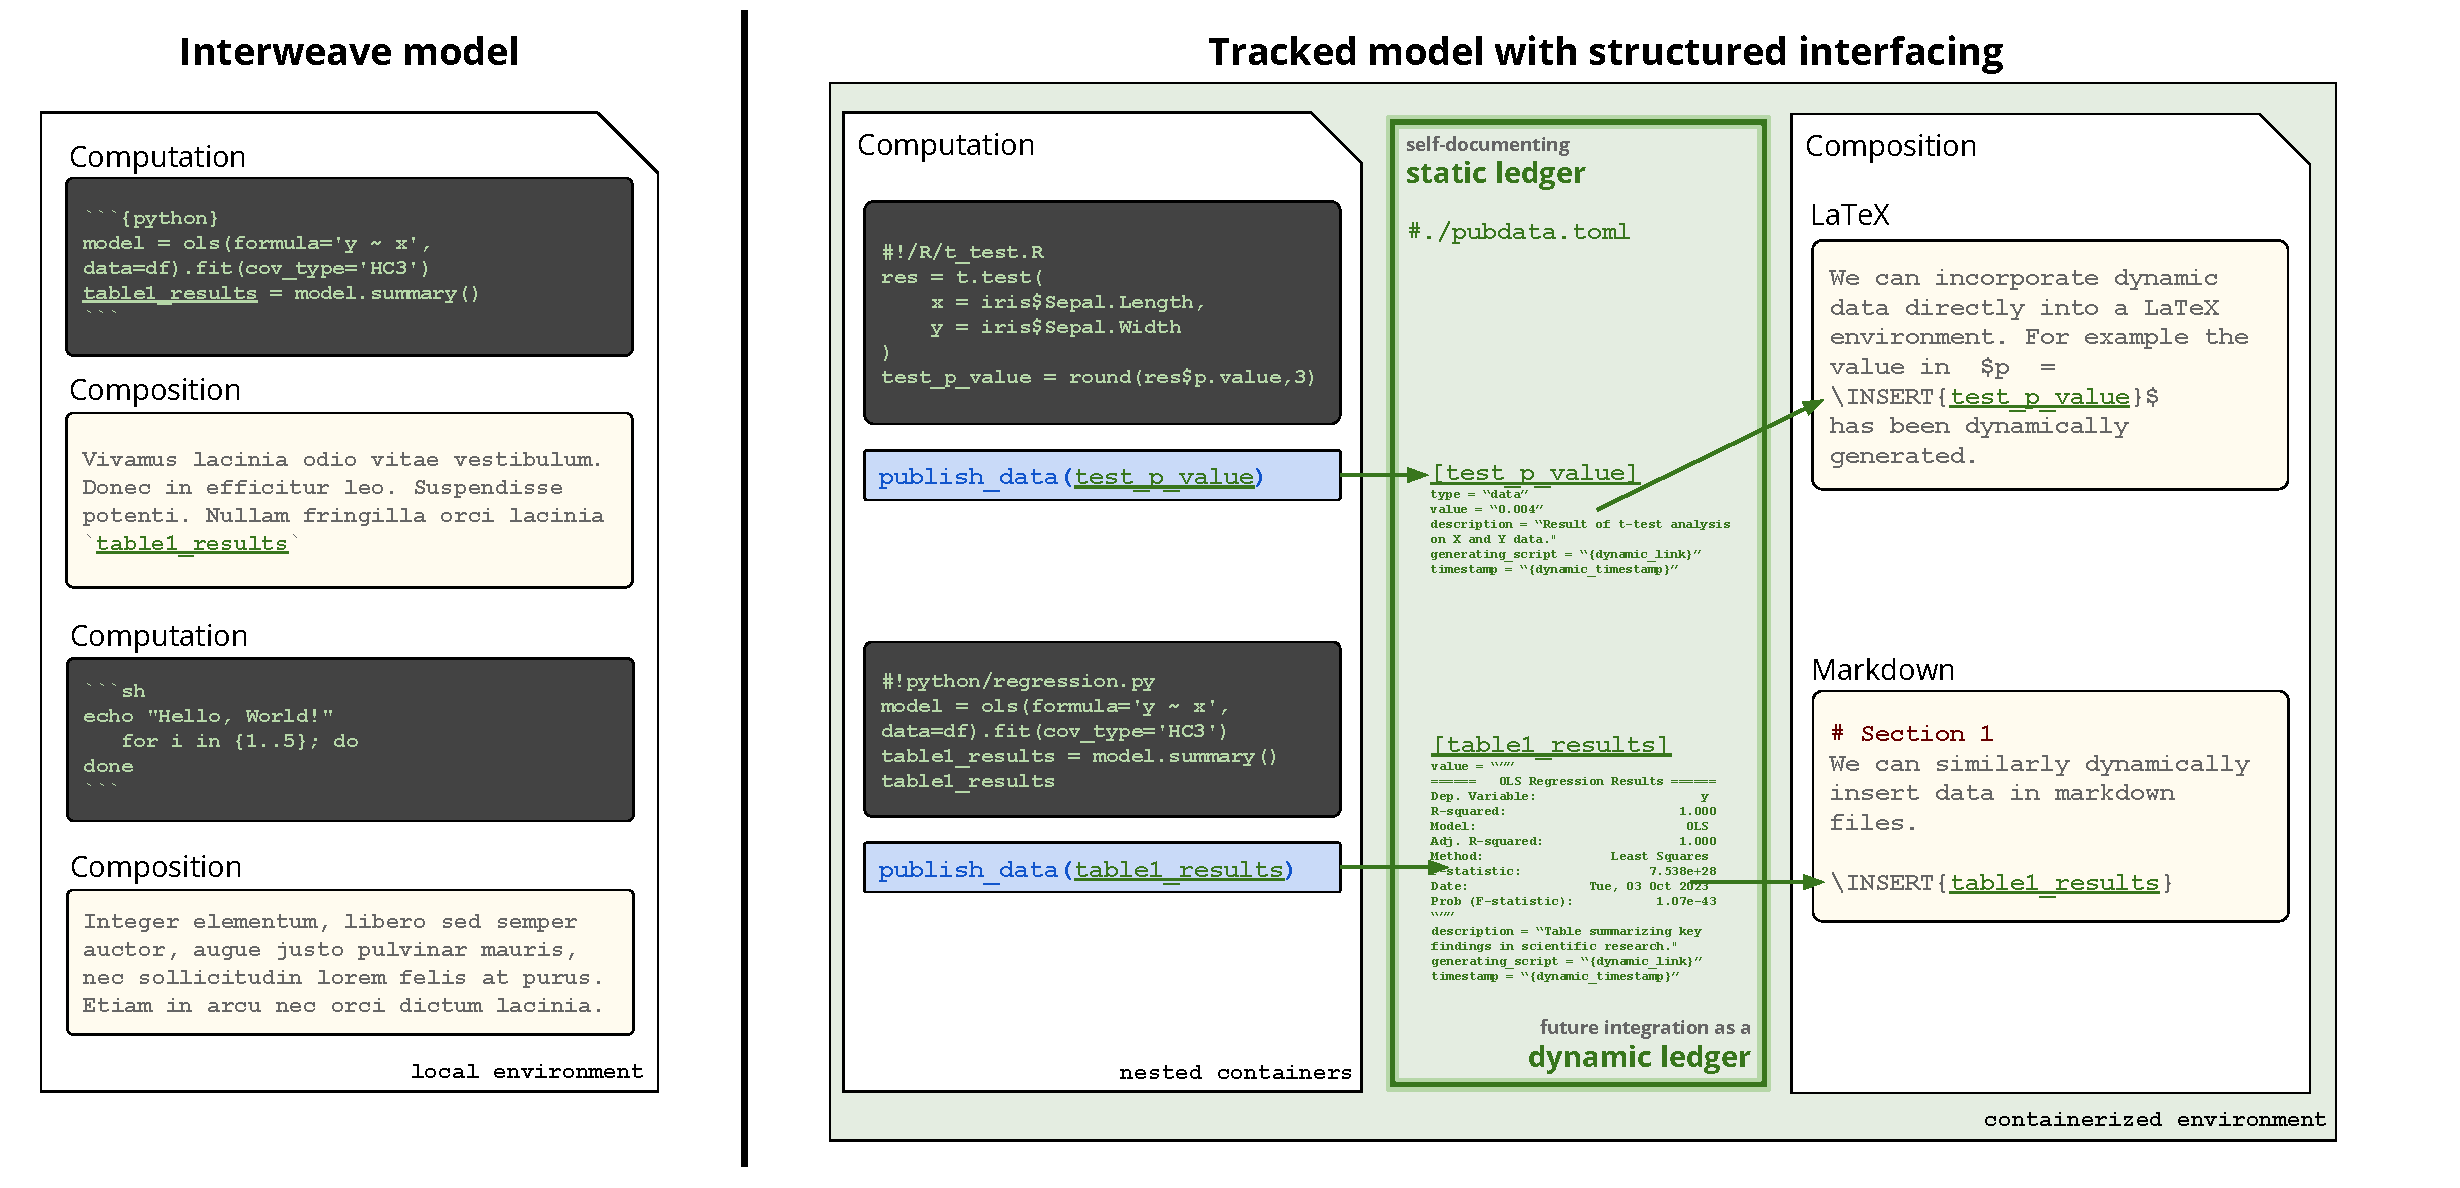
\includegraphics[width=\textwidth]{../../../../img/comp.pdf}
\vspace{2mm}
\begin{minipage}{0.95\textwidth}
%\centering
\setstretch{1}
\footnotesize{
\emph{Note:} The \textbf{interweave} model is one in which computation and composition happen linearly within the flow of a single document. Of course, existing paradigms can be quite flexible and allow for a variety of workflows; however, we believe most existing software follows this model. This leads to our proposal of the \textbf{tracked model with structured interfacing}. In this model, the data and code are tracked in a way that allows for easy verification and traceability of reported scientific results with structured metadata.
}
\end{minipage}
\end{figure}



\hypertarget{the-reproduce.work-}{%
\subsubsection{The reproduce.work \href{https://github.com/reproduce-work/sci-dev-kit}{\texttt{sci-dev-kit}}}\label{the-reproduce.work-}}

The \texttt{sci-dev-kit} is an \href{https://github.com/reproduce-work/sci-dev-kit}{open repository of code}\footnote{\href{https://github.com/reproduce-work/sci-dev-kit}{https://github.com/reproduce-work/sci-dev-kit}} that contains the basics of a reproducible scientific computing environment. It is designed to be a ``starter kit'' for scientific computing projects that are designed to be reproducible by default. Using the \texttt{sci-dev-kit} to its full potential requires the installation of \href{https://www.docker.com/}{containerization software}. Other than that, it is designed to be compatible with essentially any existing scientific workflow. 

\hypertarget{the-reproduce.work-verification-framework}{%
\subsubsection{The reproduce.work \href{}{\texttt{standards}} verification framework}\label{the-reproduce.work-verification-framework}}

The main pieces of metadata in our v0.0.1 standards framework include the following:

\begin{itemize}
\itemsep -0.2em
\item \texttt{config.toml}: A configuration file that specifies the computing environment and the software dependencies required to run the code.
\item \texttt{pubdata.toml}: A configuration file that specifies the data used in the report and the code that was used to produce the results.
\end{itemize}

With these two pieces of metadata, we are will be able to verify that the results reported in the published document are indeed reproducible. The \texttt{standards} framework is designed to be flexible and extensible, so that it can be adapted to a variety of scientific workflows. These standards currently lack many key features and will inevitably evolve over time. However, we believe that the core concept of a static ledger of structured metadata is a powerful one that can be used to facilitate the production of scientific reports that are both comprehensible and computationally reproducible.

\hypertarget{the-medium-is-the-message}{%
\subsection{The medium is the message}\label{the-medium-is-the-message}}

This document was produced using the \texttt{reproduce.work} framework; as such, we are able to automatically include and publish any data and metadata with links to the code is was used to generate any piece of data analyzed in this project. 

As an example of this phenomenon, we simulated data from a simple linear model published the data to this project's repository using the \texttt{reproduce.work} metadata standards. The data has been visuzlied in Figure \ref{fig:scatter}; this figure and the code used to generate it are also openly available in this project's repository, as can be seen by clicking on the logo in the bottom right corner of the figure.

\begin{figure}[h]
\centering
\begin{minipage}{0.75\textwidth}
\centering
\caption{A scatter plot generated using Python and compiled into this report using \texttt{reproduce.work} software}
\label{fig:scatter}
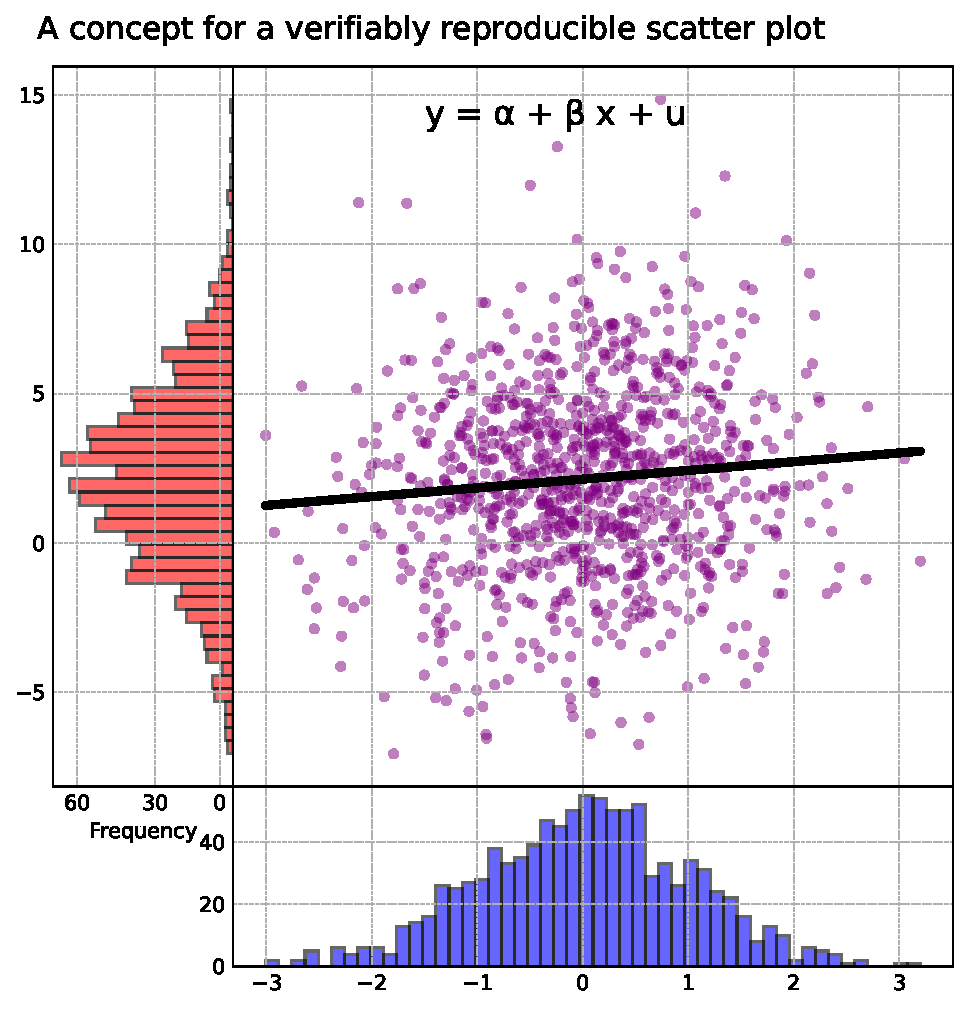
\includegraphics[width=.8\textwidth]{../../../../img/scatter_plot.pdf}
\hfill {\footnotesize \href{https://github.com/reproduce-work/reproduce-work/blob/main/reproduce/pubdata.toml}{\texttt{source} \raisebox{-1mm}{
\includegraphics[width=5mm]{../../../../img/logo.png}} }} \hspace{-1.5mm}$\;$
\end{minipage}
\end{figure}

We also include dynamic results from the output of statistical code as well, which has been embedded into this document in a way that facilitates tracing of its metadata and generating code. 

\begin{center}\begin{tabular}{r} \begin{tabular}{lcccccc} \toprule                & \textbf{coef} & \textbf{std err} & \textbf{t} & \textbf{P$> |$t$|$} & \textbf{[0.025} & \textbf{0.975]}  \\ \midrule \textbf{$\alpha$} &       2.1368  &        0.100     &    21.343  &         0.000        &        1.940    &        2.333     \\ \textbf{$\beta$}    &       0.2921  &        0.100     &     2.915  &         0.004        &        0.095    &        0.489     \\ \bottomrule \end{tabular} \\ \hfill {\footnotesize \href{https://github.com/reproduce-work/reproduce-work/blob/main/reproduce/pubdata.toml}{\texttt{source} \raisebox{-1mm}{
\includegraphics[width=5mm]{../../../../img/logo.png}} }} \hspace{-1.5mm}$\;$\end{tabular}\end{center}

The reproduce.work framework is designed to facilitate the production of scientific reports that are both human-readable and computationally reproducible. The framework is designed to be as simple as possible while accommodating a wide variety of scientific output. As an alpha version 0.0.1 example of this framework, the source code for this paper and the full stack containerized environment used to produce it are open source and can be found here run in any modern computing environment.
The aim of this paper is merely to present a proof-of-concept of the \texttt{reproduce.work} framework and demonstrate its potential for developing scientific reports. We leave the development of the framework required to reach wide adoption as an open problem for version 0.0.2 and beyond.

\hypertarget{conclusion}{%
\section{Conclusion}\label{conclusion}}

The project put forward in the body of this project is a mere first step in the direction of computational reproduction. The software lacks support for many important features and the concept is heretofore untested. While there are many aspects to reproducibility in the epistemology of science, we believe that computational reproducibility is a necessary first step toward a world where scientific results are verifiable and trustworthy. However, given the low bars required to improve the existing practices around computational reproduction, we beleive this project and the ideas put forward here have potential as the seed of a growing culture of scientific rigor and transparency.
  \newpage {\singlespacing \bibliography{bibliography} }\end{document}